\chapter{The CMS Experiment at the LHC}
\label{chapter:three}
\section{The Large Hadron Collider}

The Large Hadron Collider (LHC) is the world’s largest and most powerful particle accelerator. Inside the accelerator, two highly energetic proton beams collide up to a center-of-mass energy of 14 TeV. The LHC is constructed inside a 27 km tunnel, 100 m under the ground, located partly in Switzerland and France.

At the LHC two energetic proton beams travel in opposite directions in separate beam pipes. The proton beams travel in bunches separated by 25 ns in time. The beams travel at relativistic speeds and collide at four major interaction points at the LHC. The LHC has four main detector experiments at each interaction point: ALICE (A Large Ion Collider Experiment), ATLAS (A Toroidal LHC Apparatus), CMS (Compact Muon Solenoid), and LHCb (Large Hadron Collider beauty). ATLAS and CMS are general purpose-detectors with broad physics objectives ranging from studying the Standard Model to searching Beyond Standard Model (BSM) physics such as Dark Matter. While ALICE and LHCb are more physics dedicated detectors, ALICE and LHCb are dedicated to heavy-ion physics and studying b-quark physics respectively.
\subsection{LHC Computing Grid}
%\begin{quotation}
%    \noindent Here is a block quotation---a passage from a text you found insightful and wanted to share with others. Maybe it is from a %journal article, website, or book. Irrespective, it should support the argument being made.\footnote{A citation for the quoted material.}
%\end{quotation}

%Check appendix \ref{appendix: chapter3}

%Maybe a sentence or two that bring the argument and evidence together.\citep{dos_santos_2020}



\section{The Compact Muon Solenoid Experiment}
\subsection{Introduction}
The Compact Muon Solenoid (CMS) is a general purpose detector located in eastern France at the Large Hadron Collider (LHC) tunnel 100 m underground. It is a general purpose detector because of its broad physics searches ranging from studying the Standard Model (SM) to searching for particles that could potentially make Dark Matter (DM). CMS is a cylindrical shaped detector with 21 m in length and 15 m in cross-sectional diameter. The three main characteristics of the CMS experiment are its compactness, accurate detection of Muon particles in the muon system and its magnetic solenoid. The superconducting magnetic solenoid at the core of the CMS detector produces a continuous magnetic field of 3.8 T which is of the order of O(5) of Earth's magnetic field (0.25 - 0.65 gaus). Such large magnetic field is required for a precise measurement of the momentum of high-energy charged particles. All CMS detector subsystems are enclosed by the magnetic solenoid, the muon system, on the other hand, is on the outside. Muons are the particles that are directly detected by the CMS, with a special property that they neither stop nor decay within the boundaries of the detector. They undergo very little energy loss and thus act as a powerful medium to study high-energy process in the presence of high background.
The CMS detector is cylindrical shaped with an onion like structure, having several concentric layers of subsystems. These subsystems help prepare "photographic images" of each collision event by determining the properties of the particles in the collision. CMS has the following basic subsystems ordered from innermost to outermost:

\begin{enumerate}
    \item Silicon Tracking Detector
    \item Electromagnetic Calorimeter
    \item Hadronic Calorimeter
    \item Superconducting Solenoid Magnet
    \item Muon System
    
    
\end{enumerate}
The CMS detector can detect 5 general categories of particles as shown in the figure below:
 \begin{enumerate}
    \item Electrons
    \item Photons
    \item Charged Hadrons
    \item Neutral Hadrons
    \item Muons
\end{enumerate}

\begin{figure} [tpb]
\centering
         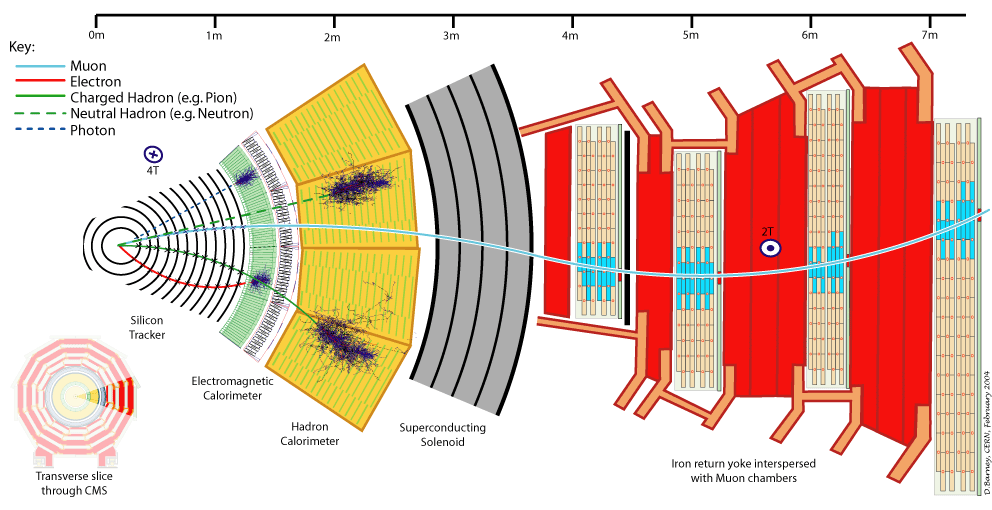
\includegraphics[width=0.9\textwidth,clip=]{thesis_template_cua/Figures/CMS_LHC_chapter/CMSSlice.png}
         \vspace*{10mm}
         \caption[CMS Slice]{This Figure shows the cross-sectional slice of the CMS detector. Here we have shown the different sub-systems of CMS, trajectories and energy deposits of the 5 general categories of particles detected by CMS by one or more of its sub-systems}
         \label{cms:slice}
\end{figure}
%More ideas that really make this a great paper. Maybe a footnote or two.\footnote{Some peripheral thoughts that belong in a note.}
\subsection{Coordinate System}
The definition of a coordinate system is very crucial in quantifying the position of a particle inside CMS with respect to the origin. CMS uses a right-handed coordinate system defined as follows and illustrated in Figure \ref{cms:coordinate} -- the origin is defined as the nominal pp collision point,  the  $x$-axis points inwards towards the center of the LHC ring, the $y$-axis points upwards perpendicular to the $x$-axis and the $z$-axis points in the counter-clockwise beam direction. However, in hadron collider physics a more traditional coordinate, pseudo-rapidity $\eta$ is used, defined as

\begin{equation}
  \eta = -\ln\tan\left(\frac{\theta}{2}\right)
  \label{eq:eta}
\end{equation}

\begin{figure} [tpb]
\centering
         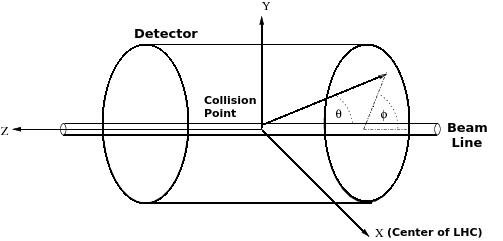
\includegraphics[width=0.9\textwidth,clip=]{thesis_template_cua/Figures/CMS_LHC_chapter/coord.png}
         \vspace*{10mm}
         \caption[CMS Coordinate System]{This Figure shows the coordinate system used by the CMS detector adapted from ~\citep{Perez:coordinate}, illustrating the $x$-axis, $y$-axis, $z$-axis, radial angle $\theta$ (measured wrt to the $z$-axis and the azimuthal angle $\phi$ (measured in $x$-$y$ plane from the $x$-axis).}
         \label{cms:coordinate}
\end{figure}

For a particle of three-momentum $\textbf{p}$ with $z$-component $p_z$, pseudorapidity can be written as
\begin{equation}
  \eta = \frac{1}{2}\ln\left(\frac{|\textbf{p}|+p_z}{|\textbf{p}|-p_z}\right)
  \label{eq:eta_p}
\end{equation}
In the limit of relativistic particles (high velocity and low mass limit), the pseudo-rapidity approximates the rapidity y given by
\begin{equation}
  y = \frac{1}{2}\ln\left(\frac{E+p_z}{E-p_z}\right),
  \label{eq:rap}
\end{equation}
The rapidity is invariant under Lorentz boost transformations and is only dependent on the polar angle $\theta$ and not on the energy of the particle. From Figure \ref{cms:rapidity}, we see that higher values of $\eta$ correspond to low values of $\theta$, this region is also referred as "forward" or high $\eta$ regions. In Figure \ref{cms:rapidity}, we observe two regions which cover approximately  $|\eta| < 1.2$ and $1.2 <|\eta|  < 3$, these regions are known as the barrel and the endcap respectively.

\begin{figure} [tpb]
\centering
         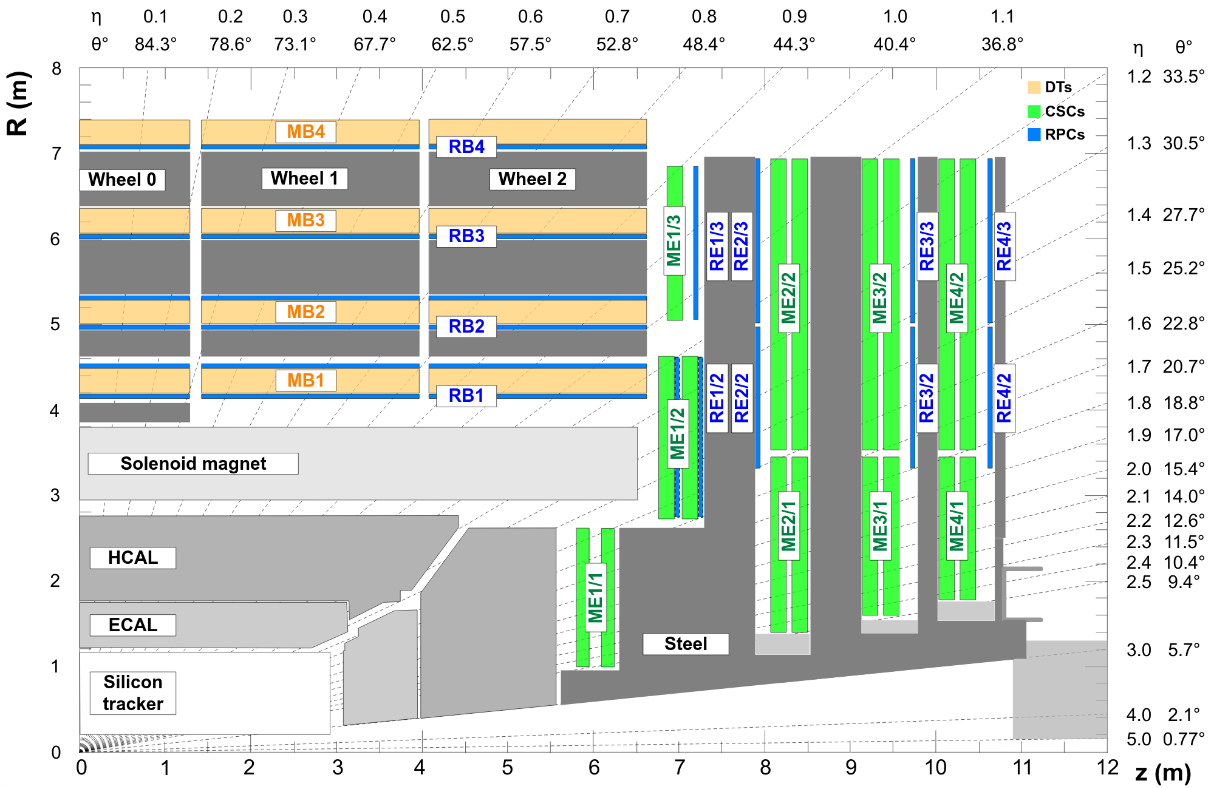
\includegraphics[width=0.9\textwidth,clip=]{thesis_template_cua/Figures/CMS_LHC_chapter/rapidity.png}
         \vspace*{10mm}
         \caption[CMS Rapidity distribution]{This Figure shows one quadrant of CMS in the $r$-$z$ plane adapted from \citep{lee:rapidity}, illustrating the positions of subsystems in barrel and endcap regions}
         \label{cms:rapidity}
\end{figure}


\subsection{Silicon Tracking Detector}
Tracking the paths of the particles produced after proton-proton collision inside CMS is of crucial importance. The tracking information from the silicon tracking detector is used to accurately reconstruct the momenta of particles such as electrons, muons or particle jets (collimated sprays of particles initiated by quarks and gluons), mitigate the effect of many overlapping proton-proton collisions (“pileup”), or correctly measure missing momentum. As the charged particles traverse the silicon sensor they create electron-hole pairs, which in the presence of an applied voltage is measured as current. 

The magnetic field is responsible for bending the charged particles, the higher the bending smaller is the momenta associated with the particles. The CMS Tracker is located inside the magnetic solenoid and is composed of two sub-systems namely, the pixel and the strip, illustrated in Figure \ref{cms:tracker} and elaborated in the following sections.

\begin{figure} [tpb]
\centering
         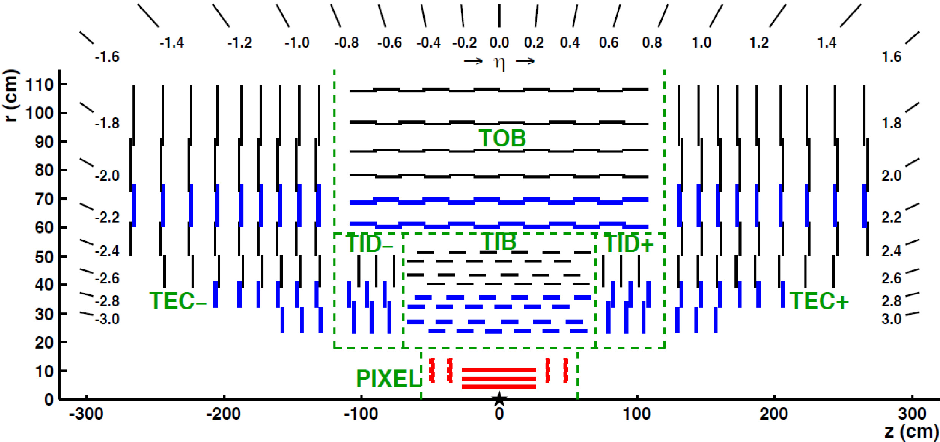
\includegraphics[width=0.9\textwidth,clip=]{thesis_template_cua/Figures/CMS_LHC_chapter/tracker.png}
         \vspace*{10mm}
         \caption[CMS Tracker r-z plane]{This Figure shows schematic of the upper half of the CMS Tracker in the $r$-$z$ plane adapted from \citep{Vormwald2016TheCI:tracker}, illustrating the positions of the pixel (red) and strip (blue).}
         \label{cms:tracker}
\end{figure}

\subsubsection{Pixel}
The Pixel sub-system is located in the high particle density region ($r<20 cm$). Being very close to the nominal proton-proton interaction point the pixel detector is exposed to most radiation. Dynamic inefficiencies like decreasing hit efficiency with increasing instantaneous luminosity, increased fake rates, reduced resolution in the inner layers as Pile up (PU) increased in the LHC, were some of the reasons which lead to the Phase I upgrade of the pixel detector. In this thesis we perform analysis of the data from all Run II years (2016, 2017, 2018) so, here we describe both the 2016 (Pixel Phase 0) and 2017/2018 (Pixel Phase I) detectors. Figure  \ref{cms:pixel} shows the layout of the 2016 (Phase 0) and 2017/2018 (Phase I) pixel detector and the geometry of the upgraded barrel layers (BPIX) and forward/backward disks (FPIX) detectors.

\begin{figure} [tpb]
\centering
         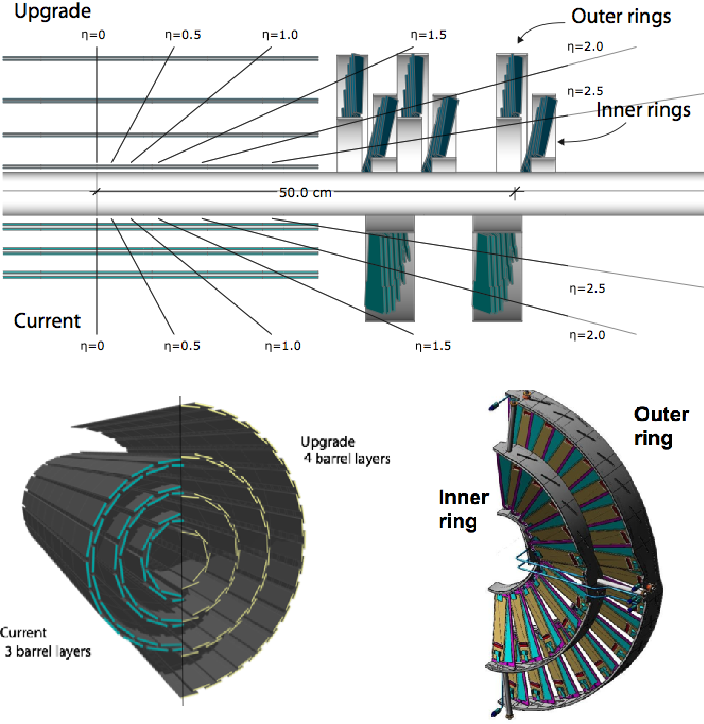
\includegraphics[width=0.9\textwidth,clip=]{thesis_template_cua/Figures/CMS_LHC_chapter/pixel_comaprision.png}
         \vspace*{10mm}
         \caption[CMS Pixel Phase 0 and Phase 1 comparison]{[Top] This Figure shows the comparison of the CMS pixel detector in Phase 0 (below center) with 3 barrel layers, 2 endcap disks and Phase 1 with 4 barrel layers, 6 endcap disks, adapted from \citep{Sakuma_2014:pixel}. [Bottom Left] figure shows the 3-D representation of 2016 (Phase 0) with 3 barrel layers and 2017/2018 (Phase 1) with 4 barrel layers. [Bottom Right] 3D placement of the inner and outer rings.}
         \label{cms:pixel}
\end{figure}
The 2016 (Phase 0) pixel \cite{CMS:2012pixel} consisted of three barrel layers (BPIX) at radii of \SI{4.4}{\cm}, \SI{7.3}{\cm} and \SI{10.2}{\cm}, and two forward/backward disks (FPIX) at longitudinal positions of $\pm$\SI{34.5}{\cm} and $\pm$\SI{46.5}{\cm} and extending in radius from about \SI{6}{\cm} to \SI{15}{\cm}. The BPIX consists of 48 million pixels covering a total area of \SI{0.78}{\meter\squared} and the FPIX has 18 million pixels covering an area of \SI{0.28}{\meter\squared}. These pixels produce a minimum of 3 independent hits along the paths of the charged particles with single hit resolutions between \SI{10}-\SI{20}{\micro\meter}.

The 2017 (Phase I) pixel \cite{Kumar2015NearFU:pixel} added an additional layer to the barrel layer and additional 4 layers to the endcap region. The layers in barrel region are arranged at radii of \SI{2.9}{\cm}, \SI{6.8}{\cm}, \SI{10.9}{\cm} and \SI{16}{\cm}. The innermost layer is made closer to the interaction point by reducing the radius of the beam pipe. The endcap region consisting of 6  layers is organized into three disks with two layers each at a distance of $\pm$\SI{29.1}{\cm}, $\pm$\SI{39.6}{\cm} and $\pm$\SI{51.6}{\cm} from the origin along the z-axis. The number of pixels in BPIX increased from 48 million to 79 million and in the FPIX region, from 18 million to 45 million covering a total area of \SI{2}{\meter\squared}. The updated tracker allows the CMS to record a minimum of 4 independent hits per track, increasing the efficiency of track reconstruction, reduced fake rates, enhanced resolution of the momentum and impact parameter at high PU.

As shown in Figure \ref{cms:pixel_sensor} the silicon sensor is composed of many layers stacked together. Each pixel unit on the sensor is bump bonded to the read-out channel on the readout-chip (ROC). These bump bonds create an electrical connection between the pixel and the readout channel on the chip. The ROC is connected via wire-bonds to the high density interconnect (HDI) for carrying the signal to the front-end electronics. The pixel sensors in the barrel are $n-on-n$ semi-conductors of size \SI{100}{\micro\meter} $\times$ \SI{150}{\micro\meter}, giving a spatial resolution of \SI{15}{\micro\meter}-\SI{20}{\micro\meter}. There are 4,160 pixels per sensor and 16 sensors per module.


\begin{figure} [tpb]
\centering
         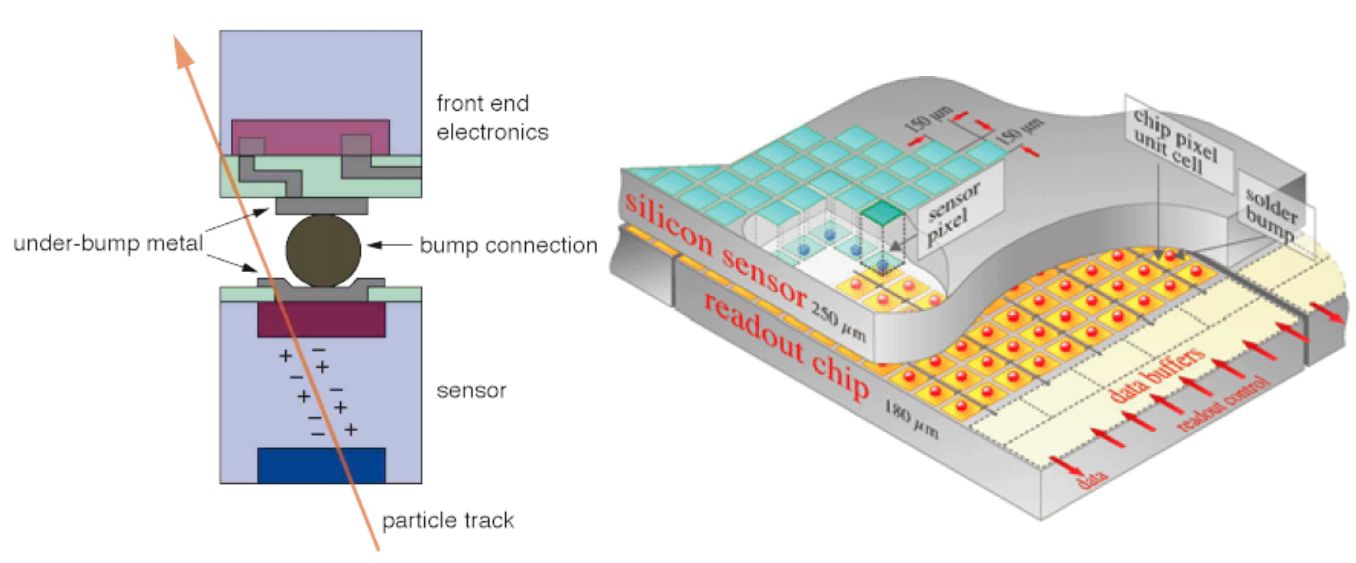
\includegraphics[width=0.9\textwidth,clip=]{thesis_template_cua/Figures/CMS_LHC_chapter/pixel_sensor.png}
         \vspace*{10mm}
         \caption[CMS Pixel sensor module]{[Left] signal read-out mechanism in a typical CMS silicon sensor. [Right] Anatomy of a silicon sensor showing distinct components like silicon bulk, ROC and bump bonds with dimensions.}
         \label{cms:pixel_sensor}
\end{figure}
\subsubsection{Strip Tracker}
The Silicon Strip Tracker (SST) surrounds the Pixel detector \cite{AGRAM2012844:strip}, the SST consists of a total of 10 layers distributed in two barrels, Tracker Inner Barrel (TIB) and Tracker Outer Barrel (TOB). The barrels are enclosed by wheels grouped into 4 parts, two Tracker Inner Disks (TIDs) with three wheels per side, two Tracker End Caps (TECs) with nine wheels per side. The SST has a diameter of \SI{2.4}{\meter} and a length of \SI{5}{\meter}. with an active area of \SI{198}{\meter\squared} distributed across 24,244 sensors it is the biggest silicon detector to be built. Figure \ref{cms:tracker} illustrates the layout of the strips.

\subsection{Electromagnetic Calorimeter}
The electromagnetic Calorimeter (ECAL) \cite{Chatrchyan:cms_detetectors} is a homogeneous and hermetic detector which measures the energy of the electromagnetically interacting particles like photons, electrons and positrons. It consists of two main components as shown in Figure \ref{cms:ecal_schema}- the barrel region composed of 61,200 lead tungstate ($PbWO_{4}$) crystals covering the region in $|\eta| < 1.479$, and the two endcap regions composed of 14,648 crystals covering the region $1.479 < |\eta|  < 3$. Avalanche photodiodes (APDs) are used in the barrel region and vacuum phototriodes (VPTs) are used in the endcap region. One of the main motivations in the design of the ECAL was its capability to detect two photons coming from the Higgs boson decay. This capability is enhanced by the good energy resolution of the ECAL.

\begin{figure} [tpb]
\centering
         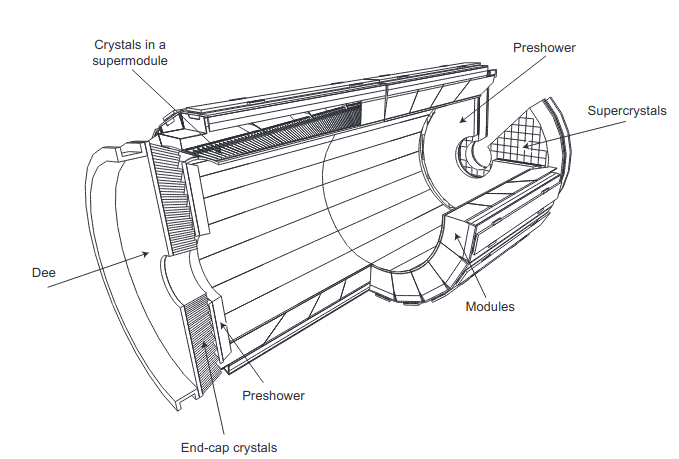
\includegraphics[width=0.9\textwidth,clip=]{thesis_template_cua/Figures/CMS_LHC_chapter/ecal_schema.png}
         \vspace*{10mm}
         \caption[CMS ECAL schema]{Schematic represntation of the CMS ECAL components adapted from \cite{Chatrchyan:cms_detetectors}}
         \label{cms:ecal_schema}
\end{figure}

The choice of $PbWO_{4}$ crystals is motivated by the following reasons. Its short radiation length (\SI{0.89}{\cm}), small $Moli\acute{e}re$ (\SI{2.19}{\cm})and high density (\SI{8.27}{\g\cm^{-3}}) results in high resolution and compactness of ECAL. It's a fast scintillator (meaning 80$\%$ of the scintillation light is emitted within 25 $ns$ of the particle's incidence on the crystal). The $PbWO_{4}$ crystals in the endcap have a truncated pyramidal shape which makes the light collection non-uniform along the crystal length. This non-uniformity is corrected by depolishing one of the lateral face of the crystal as shown in figure \ref{cms:ecal_crystal}.

\begin{figure} [tpb]
\centering
         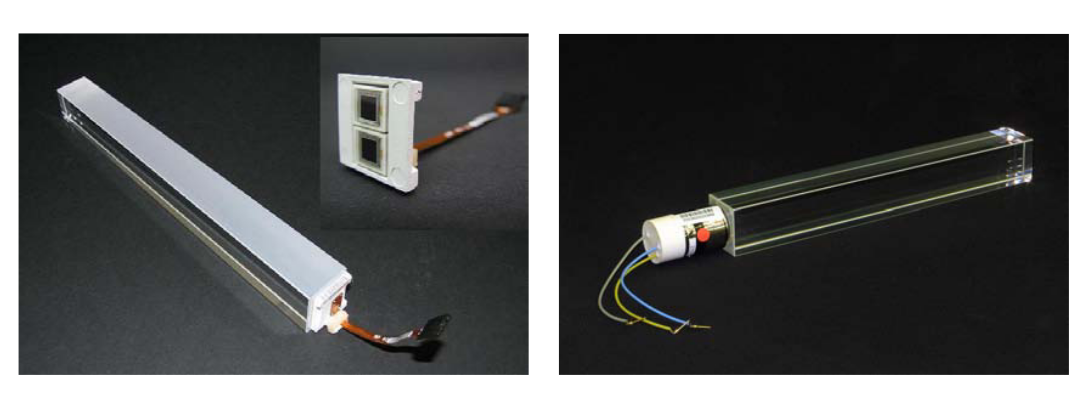
\includegraphics[width=0.9\textwidth,clip=]{thesis_template_cua/Figures/CMS_LHC_chapter/ecal_crsytal.png}
         \vspace*{10mm}
         \caption[CMS ECAL crystal]{$PbWO_{4}$ crystals with photodetectors attached.  Left panel:  A barrel crystal with the upper face depolished and the APD capsule.  In the insert, a capsule with the two APDs. Right panel: An endcap crystal and VPT}
         \label{cms:ecal_crystal}
\end{figure}

When an electron/photon traverses the ECAL crystals, it results in a cascade of electromagnetic interactions, producing a shower of particles such that the sum of there energy is proportional to the energy of the incident particle. Inside the ECAL these particles release photons which are detected by the photo-detectors at the end of the crystals. APDs (with an active area of \SI{5 x 5}{\mm}) in the barrel (two APDs per crystal) and VPTs (with an active area of \SI{280}{\mm\squared}) in the endcap (one VPT per crystal) glues at the back of the crystal as shown in Figure \ref{cms:ecal_crystal}.

The energy resolution for particles with energy below 500 GeV, the shower leakage from the rear of the calorimeter becomes significant. It is parametrized in \ref{eq:ecal_res}
\begin{equation}
\left(\frac{\sigma}{E}\right)^{2} = \left(\frac{S}{\sqrt{E}}\right)^{2} + \left(\frac{N}{E}\right)^{2} + C^{2},
  %\eta = -\ln\tan\left(\frac{\theta}{2}\right)
  \label{eq:ecal_res}
\end{equation}
where S is the stochastic term, N the noise term and C the constant term. The contribution to the stochastic term is mainly due to event-to-event fluctuations and pre-shower energy deposit fluctuations. The contribution to the noise term is due to electronics and pileup noise. Finally, the constant term is due to the non-uniform longitudinal light collection. The experimental values of these parameters were found to be 2.8\%, 0.12\% and 0.30\% for the first, second and third terms respectively. See \ref{eq:ecal_res_exp}

\begin{equation}
\left(\frac{\sigma}{E}\right)^{2} = \left(\frac{2.8\%}{\sqrt{E}}\right)^{2} + \left(\frac{0.12\%}{E}\right)^{2} + \left(0.30\%\right)^{2},
  %\eta = -\ln\tan\left(\frac{\theta}{2}\right)
  \label{eq:ecal_res_exp}
\end{equation}
\subsection{Hadronic Calorimeter}


\subsection{Solenoid Magnet}

\subsection{Muon System}

\subsection{Trigger and Data Acquisition System}

\subsection{LHC Computing Grid}
